\documentclass[a4paper, 12pt]{article}

\usepackage{/Users/zhengz/Desktop/Math/Workspace/Homework1/homework}

%%%%%%%%%%%%%%%%%%%%%%%%%%%%%%%%%%%%%%%%%%%%%%%%%%%%%%%%%%%%%%%%%%%%%%%%%%%%%%%%%%%%%%%%%%%%%%%%%%%%%%%%%%%%%%%%%%%%%%%%%%%%%%%%%%%%%%%%
\begin{document}
%Header-Make sure you update this information!!!!
\noindent
%%%%%%%%%%%%%%%%%%%%%%%%%%%%%%%%%%%%%%%%%%%%%%%%%%%%%%%%%%%%%%%%%%%%%%%%%%%%%%%%%%%%%%%%%%%%%%%%%%%%%%%%%%%%%%%%%%%%%%%%%%%%%%%%%%%%%%%%
\large\textbf{Zhengdong Zhang} \hfill \textbf{Homework 1}   \\
Email: zhengz@uoregon.edu \hfill ID: 952091294 \\
\normalsize Course: MATH 635 - Algebraic Topology II \hfill Term: Winter 2025\\
Instructor: Dr.Daniel Dugger \hfill Due Date: $13^{th}$ January, 2024 \\
\noindent\rule{7in}{2.8pt}
\setstretch{1.1}
\begin{problem}{1}
The following turns out to be a complete list of all compact 2-manifold:
\[S^2,T,T\# T,T\#T\#T,\ldots, \mathbb{R}P^2, \mathbb{R}P^2\#\mathbb{R}P^2,\mathbb{R}P^2\#\mathbb{R}P^2\#\mathbb{R}P^2,\ldots\]
Compute the homology groups and Euler characteristics for each of them.
\end{problem}
\begin{solution}

\begin{enumerate}[(1)]
\item 2-sphere \(S^2\).

For the 2-sphere \(S^2\), it has a CW structure with only one 0-cell and one 2-cell. So the boundary map is all zero and the CW chain complex is as follows: 
\[\mathbb{Z}\xrightarrow{0} 0\xrightarrow{0} \mathbb{Z}.\]
So we have 
\[H_i(S^2)=\begin{cases}
    \mathbb{Z},&\ \text{if}\  i=0,2;\\ 
    0,&\ \text{otherwise}.
\end{cases}\]
The Euler characteristics is 
\[\chi(S^2)=\rank H_0(S^2)+\rank H_2(S^2)=2.\]
\item Torus \(T\) and real projective space \(\mathbb{R}P^2\). 

Consider the following CW structure:
\begin{figure}[h]
    \centering
    \begin{minipage}[b]{0.4\textwidth}
      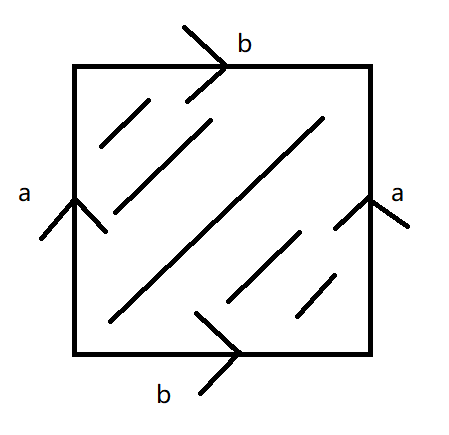
\includegraphics[width=0.7\textwidth]{Pictures/HW1-1-1.png}
      \caption{\(T\)}
    \end{minipage}
    \hfill
    \begin{minipage}[b]{0.4\textwidth}
      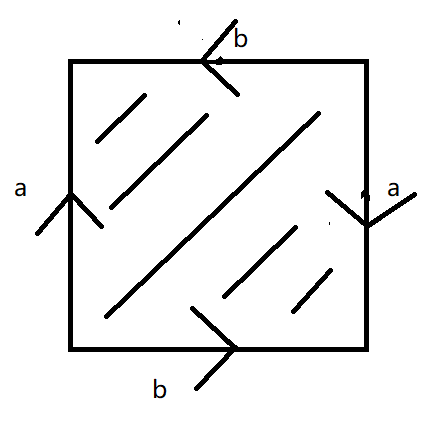
\includegraphics[width=0.7\textwidth]{Pictures/HW1-1-2.png}
      \caption{\(\mathbb{R}P^2\)}
    \end{minipage}
  \end{figure}
The torus \(T\) has one 0-cell \(x\), two 1-cells \(a\) and \(b\), one 2-cell \(S\). We have the following cellular chain complex:
\[\mathbb{Z}\xrightarrow{d_2}\mathbb{Z}^2\xrightarrow{d_1}\mathbb{Z}.\]
The boundary map \(d_1=0\) since we only have one 0-cell. From the figures above, we know that for the torus \(T\), we have 
\[d_2(S)=a+b-a-b=0.\]
So for the torus \(T\), we have 
\[H_i(T)=\begin{cases}
    \mathbb{Z},&\ \text{if}\ i=0,2;\\ 
    \mathbb{Z}^2,&\ \text{if}\ i=1;\\ 
    0,&\ \text{otherwise}.
\end{cases}\]
The Euler characteristics is 
\[\chi(T)=\rank H_0(T)-\rank H_1(T)+\rank H_2(T)=0.\]

For the real projective space \(\mathbb{RP}^2\), we have two 0-cells \(x,y\), two 1-cells \(a,b\) and one 2-cell \(S\). The cellular chain complex is as follows:
\[\mathbb{Z}\xrightarrow{d_2}\mathbb{Z}^2\xrightarrow{d_1}\mathbb{Z}^2.\]
The boundary map \(d_2\) sends \(S\) to 
\[d_2(S)=2a-2b\]
and the boundary map 
\begin{align*}
    d_1(a)&=x-y,\\
    d_1(b)&=x-y.
\end{align*}
So we can calculate the homology groups 
\begin{align*}
    H_0(\mathbb{R}P^2)&=\ker d_0/\im d_1\\ 
                      &=\la x,y\ra/\la x-y\ra\\ 
                      &=\la x-y,y\ra/\la x-y\ra\\ 
                      &=\mathbb{Z}.
\end{align*}
and 
\begin{align*}
H_1(\mathbb{R}P^2)&=\ker d_1/\im d_2\\ 
                  &=\la a-b\ra/\la 2a-2b\ra\\ 
                  &=\mathbb{Z}/2 \mathbb{Z}
\end{align*}   
So we have 
\[H_i(\mathbb{R}P^2)=\begin{cases}
    \mathbb{Z},&\ \text{if}\ i=0;\\ 
    \mathbb{Z}/2 \mathbb{Z},&\ \text{if}\ i=1;\\ 
    0,&\ \text{otherwise}.
\end{cases}\]
The Euler characteristics is 
\[\chi(\mathbb{R}P^2)=\rank H_0(\mathbb{RP}^2)-\rank H_1(\mathbb{R}P^2)=1.\]
\item The following pictures give CW structures to the connected sum \(T\# T\) and \(\mathbb{R}P^2\#\mathbb{R}P^2\):
\[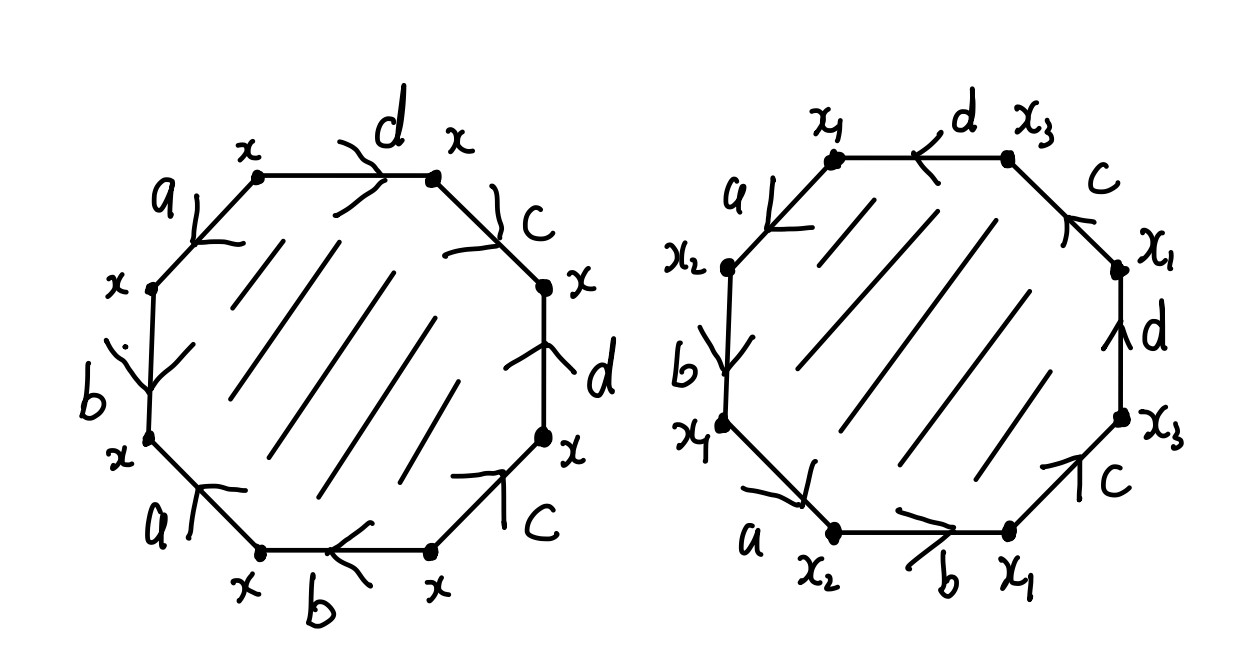
\includegraphics[scale=0.5]{Pictures/HW1-1-3.png}\]
Note that for the connected sum of tori \(T\#T\), we have one 0-cell, four 1-cell and one 2-cell, and for the connected sum of real projective space, we have three 0-cells, four 1-cells and one 2-cell. These CW structures can be generalized to \(n\)-copies of 
connected sum \(T\#T\#\cdots \#T\) and \(\mathbb{R}P^2\#\mathbb{R}P^2\#\cdots\#\mathbb{R}P^2\). 
\begin{itemize}
\item For \(T\#T\#\cdots\#T\), we have one 0-cell \(x\), \(2n\) 1-cells \(a_1,b_1,a_2,b_2,\ldots,a_n,b_n\) and one 2-cell \(S\). The celluar chain complex is given by 
\[\mathbb{Z}\xrightarrow{d_2}\mathbb{Z}^{2n}\xrightarrow{d_1} \mathbb{Z}\]
where 
\[d_2(S)=(a_1+b_1-a_1-b_1)+(a_2+b_2-a_2-b_2)+\cdots+(a_n+b_n-a_n-b_n)=0\]
and \(d_1=0\) since we only have one 0-cell. So the homology group is given by 
\[H_i(T\#T\#\cdots\#T)=\begin{cases}
    \mathbb{Z},&\ \text{if}\ i=0,2;\\
    \mathbb{Z}^{2n},&\ \text{if}\ i=1;\\ 
    0,&\ \text{otherwise}. 
\end{cases}\]
The Euler characteristics is 
\[\chi(T\#T\#T\cdots\# T)=1-2n+1=2-2n.\]
\item For \(Y=\mathbb{R}P^2\#\mathbb{R}P^2\#\cdots\#\mathbb{R}P^2\), we have \(n+1\) 0-cells \(x_1,x_2,\ldots,x_{n+1}\), \(2n\) 1-cells \(a_1,b_1,a_2,b_2,\ldots,a_n,b_n\) and one 2-cell \(S\). The cellular complex is given by 
\[\mathbb{Z}\xrightarrow{d_2}\mathbb{Z}^{2n}\xrightarrow{d_1}\mathbb{Z}^{n+1}\]
where 
\[d_2(S)=2(a_1+b_1+\cdots+a_n+b_n)\]
and 
\[d_1(a_i)=x_{i+1}-x_i=-d_1(b_i)\]
for \(1\leq i\leq n+1\) and assume \(x_{n+2}=x_1\). We can see that \(\ker d_2=0\) so \(H_2(Y)=0\). And 
\begin{align*}
    H_0(Y)&=\ker d_0/\im d_1\\ 
          &=\la x_1,x_2,\ldots,x_{n+1}\ra/\la x_2-x_1,x_3-x_2,\ldots,x_{n+1}-x_n\ra\\ 
          &=\la x_1\ra\\ 
          &=\mathbb{Z}. 
\end{align*}
\begin{align*}
    H_1(Y)&=\ker d_1/\im d_2\\ 
          &=\la a_1+b_1,a_2+b_2,\ldots,a_n+b_n\ra/\la 2(a_1+b_1+\cdots a_n+b_n)\ra\\ 
          &=\la (a_1+b_1+\cdots+a_n+b_n),a_2+b_2,\ldots,a_n+b_n\ra/\la 2(a_1+b_1+\cdots a_n+b_n)\ra\\ 
          &=\mathbb{Z}/2 \mathbb{Z}\oplus \mathbb{Z}^{n-1}.
\end{align*}
So the homology group of \(Y=\mathbb{R}P^2\#\cdots \# \mathbb{R}P^2\) with \(n\) copies of \(\mathbb{R}P^2\) can be summarized as follows:
\[H_i(Y)=\begin{cases}
    \mathbb{Z},&\ \text{if}\ i=0;\\ 
    \mathbb{Z}/2 \mathbb{Z}\oplus \mathbb{Z}^{n-1},&\ \text{if}\ i=1;\\ 
    0,&\ \text{otherwise}.
\end{cases}\]
The Euler characteristics is 
\[\chi(Y)=1-(n-1)=2-n.\]
\end{itemize}
\end{enumerate}
\end{solution}

\noindent\rule{7in}{2.8pt}


\begin{background}
The remaining exercises will hep you get started towards a proof that all compact 2-manifolds are as stated in problem 1.

Suppose one has  polygon with labelled edges, representing a quotient space. Assume every edge is labelled, and every label occurs exactly twice. Such a quotient 
space is a 2-dimensional manifold. 
If we have a diagram such as 
\[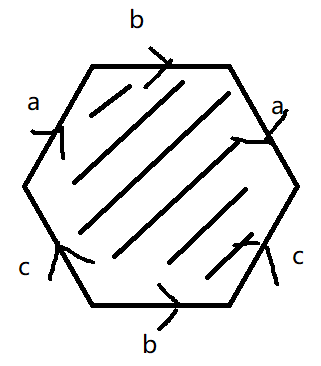
\includegraphics[scale=0.5]{Pictures/HW1-1.png}\]
we will represent this by the string "\(abac^{-1}b^{-1}c\)". Notice that we could also represent it by the string "\(b^{-1}cabac^{-1}\)", as well as others. When talking about these 
strings I will use letters \(x,y,z\) to stand for one symbol (like \(a\) or \(a^{-1}\))and letters \(A,B,C\) to stand for a block of symbols (like \(aba\) or \(c^{-1}b^{-1}\)).

If \(B\) is a block \(x_1x_2\cdots x_k\), let \(B^{-1}\) denote the block \(x_k^{-1}x_{k-1}^{-1}\cdots x_1^{-1}\). Our convention is that \((x^{-1})^{-1}=x\) so that for instance if \(B\) is the block \(abc^{-1}\) then 
\(B^{-1}\) is \(cb^{-1}a^{-1}\).

We will say that two strings are equivalent if the corresponding quotient spaces are homeomorphic. Here are some basic cases of equivalent strings. 
\begin{enumerate}[(i)]
\item The strings \(x_1x_2\cdots x_n\) and \(x_nx_1x_2 \cdots x_{n-1}\) are equivalent. 
\item If you insert \(xx^{-1}\) or \(x^{-1}x\) into any string which does not have an \(x\), you get an equivalent string. [Taking this and working backwards, if you remove either \(xx^[-1]\) or \(x^-1x\) from a given string then you get an 
equivalent one.]
\item The string \(ABCBD\) is equivalent to \(AxCxD\), assuming the letter \(x\) does not appear in \(A,C\) or \(D\). (That is, if a block occurs twice then we can rename the whole block to just one letter). Likewise, the string \(ABCB^{-1}D\) is equivalent to \(AyCy^{-1}D\).
\end{enumerate}
Based on all this, we do the following exercises.
\end{background}

\begin{problem}{3}
Using (i)-(iii), explain why a string \(AC\) is equivalent to both \(ABB^{-1}C\) and \(AB^{-1}BC\), assuming that none of the letters in \(B\) appears in \(AC\).
\end{problem}
\begin{solution}
Note that \((BB^{-1})^{-1}=B^{-1}B\), we only need to prove that \(ABB^{-1}C\) is equivalent to \(AC\). The other situation is just by replacing \(B\) with \(B^{-1}\). Let \(x\) be a letter that does not appear in \(A,B,C\), by (ii), we have 
\(ABB^{-1}C\cong AB(xx^{-1})B^{-1}C\). Denote the block \(xx^{-1}\) by \(D\), by (iii), we have 
\[ABDB^{-1}C\cong AyDy^{-1}C\cong Ayxx^{-1}y^{-1}C\cong A(yx)(yx)^{-1}C\cong AC\]
since none of the letters in \(B\) appears in \(A\) and \(C\), so both \(x\) and \(y\) does not appear in \(A\) and \(C\).
\end{solution}

\noindent\rule{7in}{2.8pt}


\begin{problem}{4}
Use a topological cut-and-paste arguments, prove that \(AxBCxD\) is equivalent to \(AyCyB^{-1}D\). Also prove that \(AxBCx^{-1}D\) is equivalent to \(AyCBy^{-1}D\), and \(ABxCx^{-1}D\) is equivalent to 
\(AyCy^{-1}BD\).
\end{problem}
\begin{solution}
We cut open along the red line \(y\) and paste along \(x\) as shown in the following picture:
\[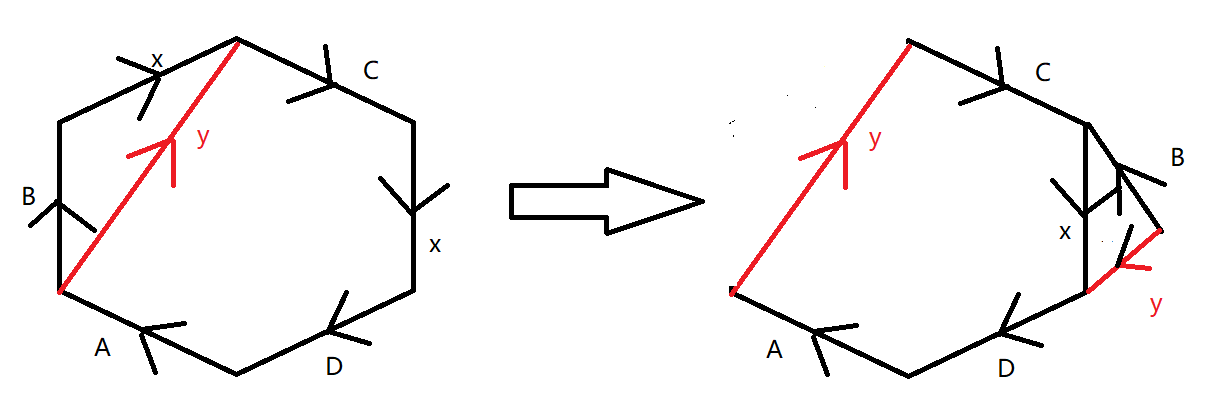
\includegraphics[scale=0.5]{Pictures/HW1-4.png}\]
This proves that the string \(ABxCxD\) is equivalent to \(AyCB^{-1}yD\).
\end{solution}

\noindent\rule{7in}{2.8pt}

\begin{problem}{5}
Again using topological cut-and-paste arguments, prove that \(AxBCxD\) is equivalent to \(AyCyB^{-1}D\). Also prove that \(AxBCx^{-1}D\) is equivalent to \(AyCBy^{-1}D\), and \(ABxCx^{-1}D\) is equivalent to \(AyCy^{-1}BD\).
\end{problem}
\begin{solution}
The cut and paste procedure is shown in the following pictures:
\[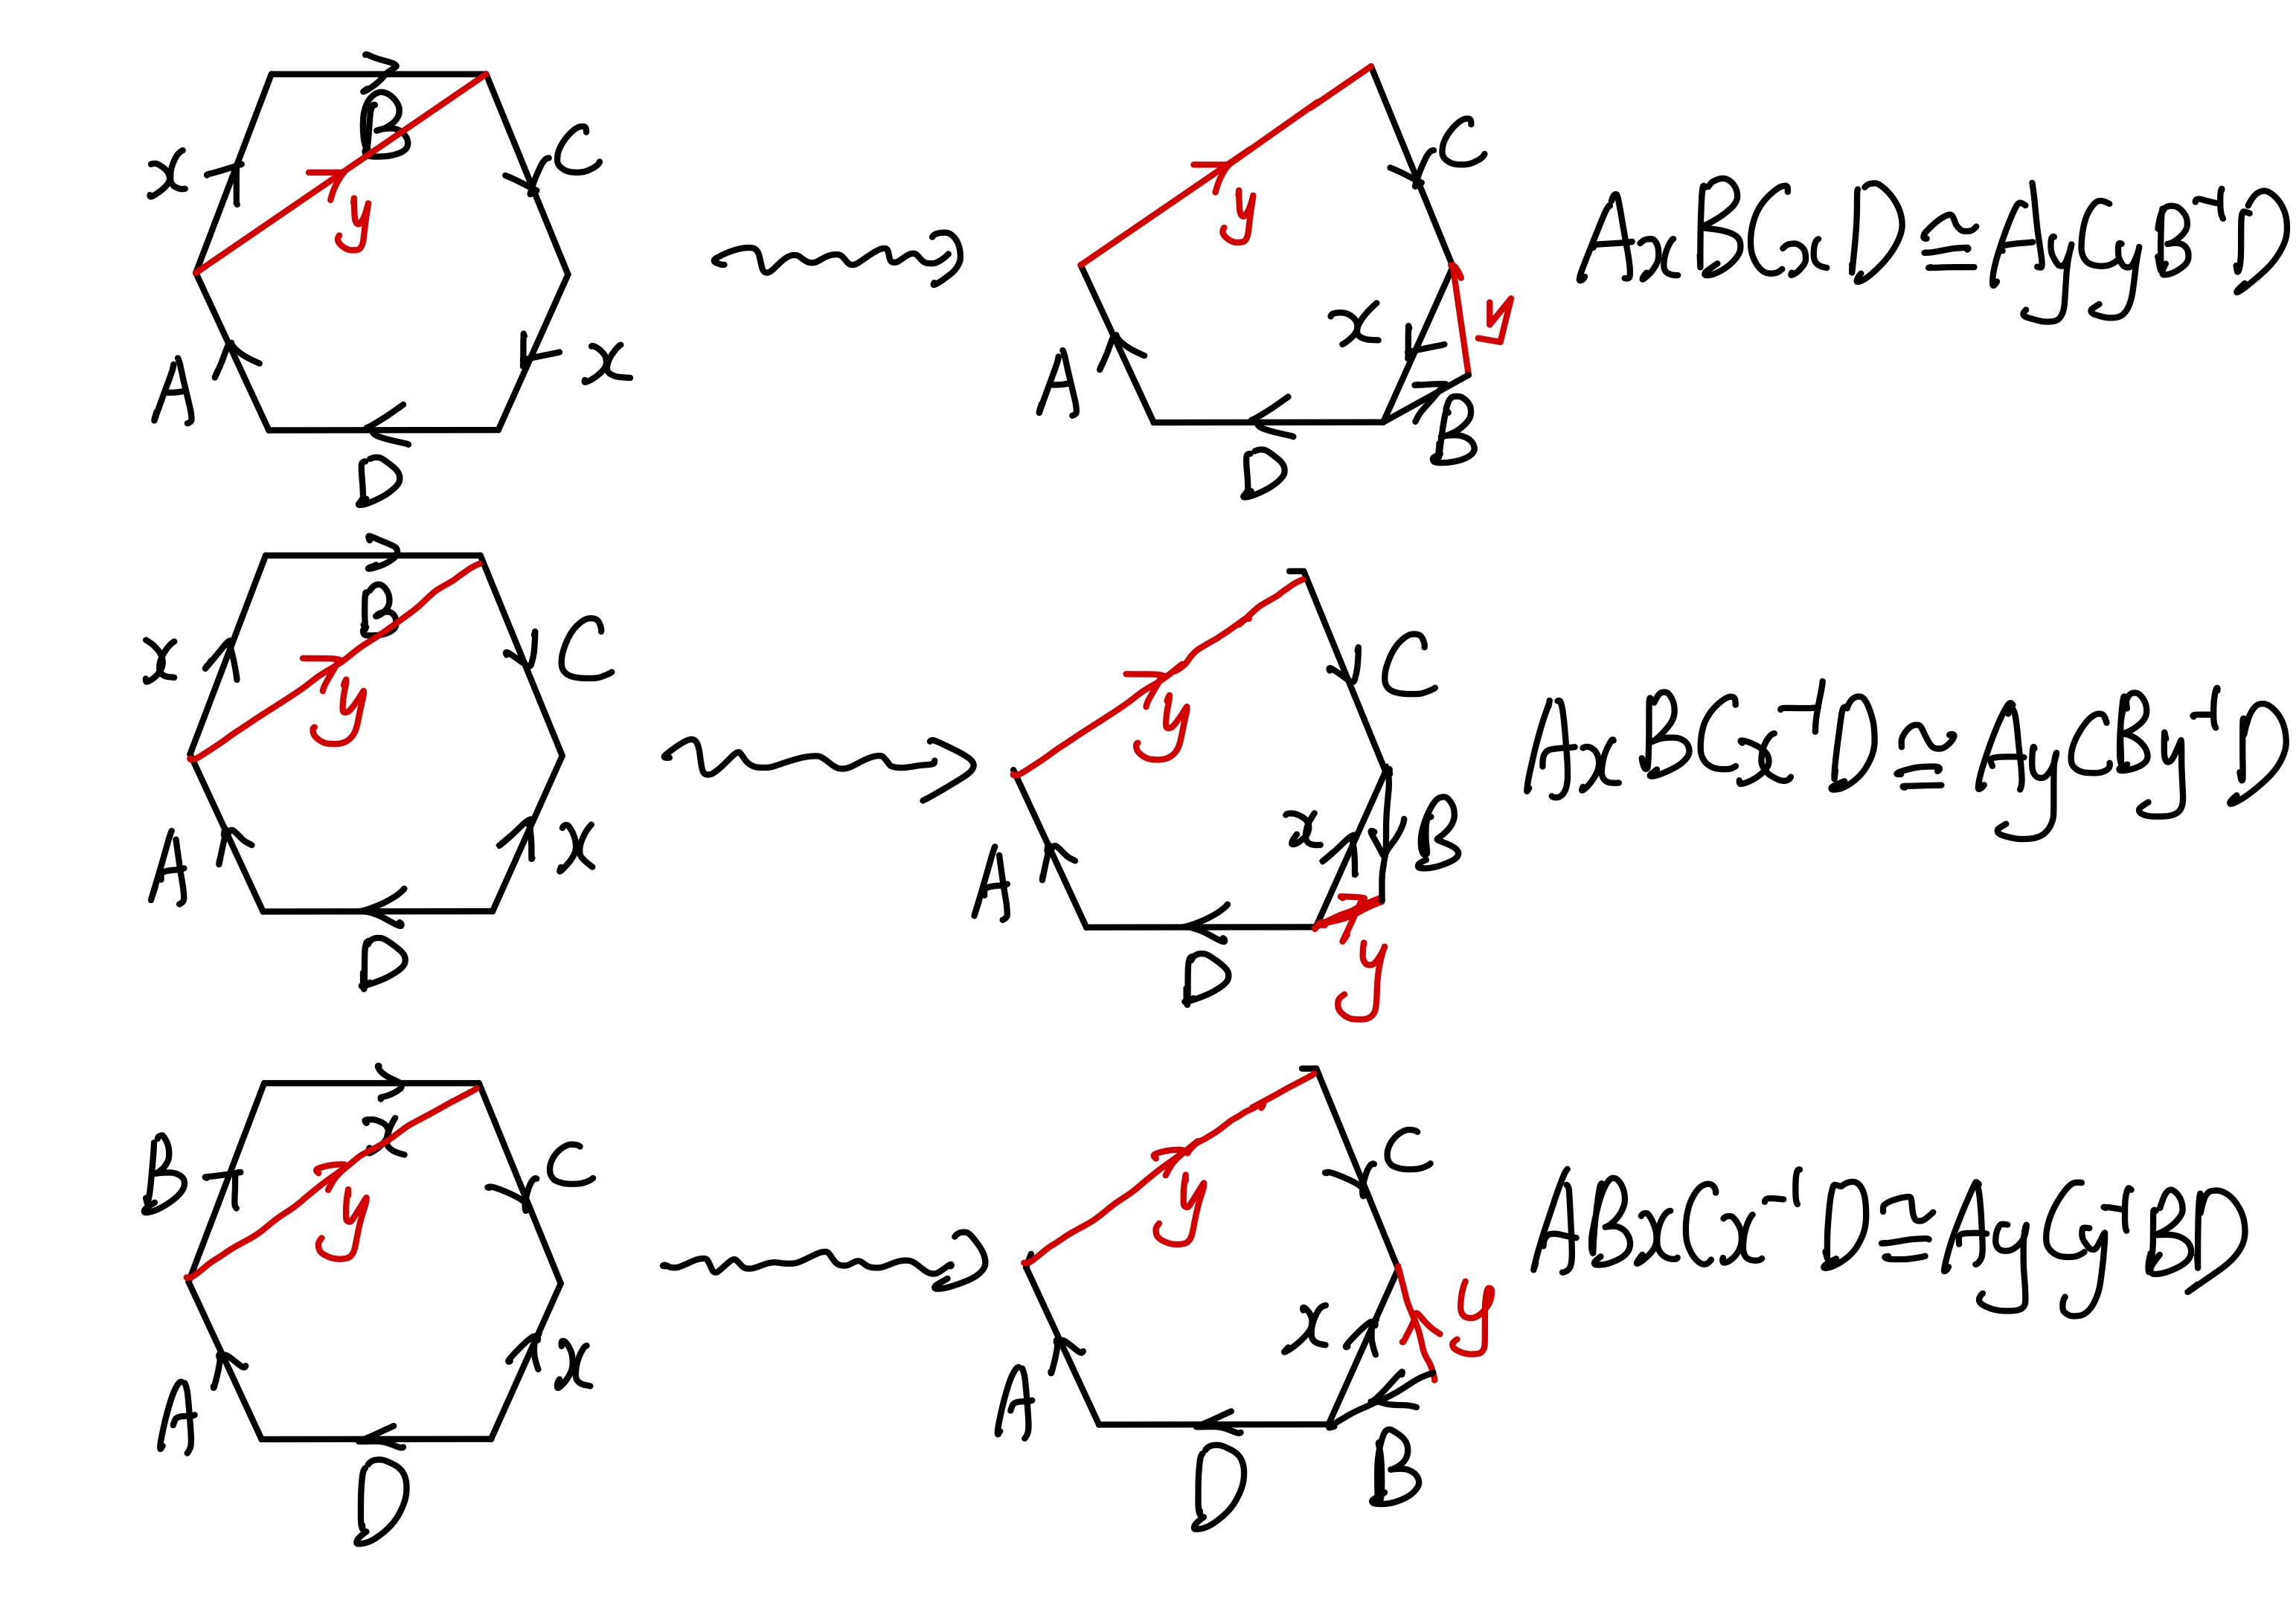
\includegraphics[scale=0.1]{Pictures/HW1-5.jpg}\]
\end{solution}

\noindent\rule{7in}{2.8pt}

\begin{background}
We can summarize the rules you've established in question 2-4 as follows:
\begin{enumerate}[(1)]
\item \(AxBCxD\sim AxCxB^{-1}D\)
\item \(ABxCxD\sim AxCB^{-1}xD\)
\item \(AxBCx^{-1}D\sim AxCBx^{-1}D\)
\item \(ABxCx^{-1}D\sim AxCx^{-1}BD\) 
\end{enumerate}
The rules can be paraphrased as follows:
\begin{itemize}
\item If \(x\) occurs twice in a string (without any inverse on it), then a block next to the first \(x\) can be moved to a block on the same side of the second \(x\), but the new block has to be inverted.
\item If \(x\) and \(x^{-1}\) occur in a string, then a block next to the first one can be moved to a block on the other side of the second on , and the block does not get inverted. 
\end{itemize}
As an example of using these rules, we can write 
\[abacb^{-1}ddc\sim abacdbdc\sim cdbda^{-1}b^{-1}a^{-1}c\sim cdabda^{-1}b^{-1}c.\]
\end{background}

\begin{problem}{6}
Using (i)-(iii) and (1)-(4), prove the following equivalences:
\begin{enumerate}[(a)]
\item \(abab\sim xx\).
\item \(abab^{-1}\sim xxyy\). (This shows that \(K\cong \mathbb{R}P^2\#\mathbb{R}P^2\))
\item \(aabcb^{-1}c^{-1}\sim xxyyzz\). (This shows that \(\mathbb{R}P^2\# T\cong \mathbb{R}P^2\# \mathbb{R}P^2\# \mathbb{RP}^2\))
\end{enumerate}
\end{problem}
\begin{solution}
\begin{enumerate}[(a)]
\item Use (iii). Assume \(A,C,D\) are empty blocks and \(B=ab\). We have \(abab\sim xx\).
\item First we use Rule (1) with \(A=D\) is the empty block, \(x=a\), \(C=b\) and \(B^{-1}=b^{-1}\), so we have \(abab^{-1}\sim abba\). Then (i) and this tells us \(abab^{-1}\sim abba\sim aabb\).
\item First rewrite \(aabcb^{-1}c^{-1}\) into \(abcb^{-1}c^{-1}a\) using (i). Then use use Rule (2) with \(A,D\) empty, \(x=a\), \(C=bc\), and \(B=cb\), we have 
\[abcb^{-1}c^{-1}a\sim cbabca.\]
Then use Rule (2) with \(A=c\), \(x=b\), \(C\) empty, \(B=a^{-1}\) and \(D=ca\), we have 
\[cbabca\sim ca^{-1}bbca\sim caca^{-1}bb.\]
Use Rule (2) with \(A,C\) empty, \(B=a^{-1}\) and \(D=a^{-1}bb\), we have 
\[caca^{-1}bb\sim a^{-1}cca^{-1}bb.\]
Finally use Rule (2) with \(A,C\) empty, \(B=c^{-1}c^{-1}\), \(x=a^{-1}\) and \(D=bb\), we have 
\[c^{-1}c^{-1}a^{-1}a^{-1}bb.\]
Let \(c^{-1}=x\), \(a^{-1}=y\) and \(b=z\) and we are done.
\end{enumerate}
\end{solution}

\noindent\rule{7in}{2.8pt}

\begin{problem}{7}
Now we turn to the classification of compact 2-manifolds. Note that \(S^2\) is represented by the string \(xx^{-1}\), which is equivalent to the empty string.

Let \(S\) be a string of letters and their 'inverse', in which each letter appears twice (meaning either twice as itself or once as \(x\) and once as \(x^{-1}\)). Use (i)-(iii) and (1)-(4) to do the following:
\begin{enumerate}[(a)]
\item Prove that if a letter \(x\) appears twice as itself, then \(S\) is equivalent to a string in which \(xx\) appears as the beginning. [That is, prove that \(AxBxC\sim xxD\), for some block \(D\)]
\item Prove that a string of the form \(AsCtDs^{-1}Et^{-1}\) is equivalent to one which starts out as \(sts^{-1}t^{-1}\).
\item Let \(M\) be the 2-dimensional manifold corresponding to the string 
\[abca^{-1}befe^{-1}c^{-1}f.\]
Determine which of the 2-manifold is homeomorphic to \(M\).
\item Repeat part (c) for the manifold correponding to 
\[dbced^{-1}c^{-1}e^{-1}b^{-1}.\]
\item Explain why any string of the form 
\[a_1a_1a_2a_2\cdots a_ka_ks_1t_1s_1^{-1}t^{-1}\cdots s_rt_rs_r^{-1}t_r^{-1}\]
in which \(k\geq 1\) is equivalent to one of the form 
\[b_1b_1b_2b_2\cdots b_nb_n.\]
\item Think about how you would prove that any string is equivalent to either one of the form 
\[a_1a_1a_2a_2\cdots a_ka_k\]
or 
\[s_1t_1s_1^{-1}t_1^{-1}\cdots s_rt_rs_r^{-1}t_r^{-1}.\]
\end{enumerate}
\end{problem}
\begin{solution}
\begin{enumerate}[(a)]
\item Given a string \(AxBxC\), use Rule (1), we have 
\[AxBxC\sim AxC^{-1}Bx\sim xC^{-1}BxA\sim xA^{-1}C^{-1}Bx\sim xxA^{-1}C^{-1}B\sim xxD\]
where \(D=A^{-1}C^{-1}B\).
\item First we use Rule (4) with \(A=A\), \(x=s\), \(C=CtD\), \(B=E\) and \(D=t^{-1}\), we have 
\[AsCtDs^{-1}Et^{-1}\sim AEsCtDs^{-1}t^{-1}.\]
Then use Rule (4) again with \(A=AEs\), \(B=C\), \(x=t\), \(C=Ds^{-1}\),\(D\) empty, we have 
\[AEsCtDs^{-1}t^{-1}\sim AEstDs^{-1}t^{-1}C.\]
Next use Rule (3) with \(A=AEs\), \(x=t\),\(B=D\),\(C=s^{-1}\), \(D=C\), we have 
\[AEstDs^{-1}t^{-1}C\sim AEsDts^{-1}t^{-1}C.\]
Finally use Rule (4) again with \(A=AEs\), \(x=t\), \(B=D\), \(C=s^{-1}\) and \(D=C\), we have 
\[AEsDts^{-1}t^{-1}C\sim AEsts^{-1}t^{-1}DC\sim sts^{-1}t^{-1}DCAE.\]
\item First let \(A=a\), \(x=b\), \(B=ca^{-1}\) and \(C=efe^{-1}c^{-1}f\). Use (a), then 
\[D=A^{-1}C^{-1}B=a^{-1}f^{-1}cef^{-1}e^{-1}ac^{-1}\]
and the original string equals to 
\[bba^{-1}f^{-1}cef^{-1}e^{-1}ac^{-1}\]
Use part (a) again with \(A=bba^{-1}\), \(x=f^{-1}\), \(B=ce\) and \(C=e^{-1}ac^{-1}\), this time the string becomes
\[f^{-1}f^{-1}A^{-1}C^{-1}B=f^{-1}f^{-1}ab^{-1}b^{-1}ca^{-1}ece.\]
Use part (a) again with \(A=f^{-1}f^{-1}ab^{-1}b^{-1}\), \(x=c\), \(B=a^{-1}e\) and \(C=e\), the string becomes 
\[ccbba^{-1}ffe^{-1}a^{-1}e\]
Use part (a) again with \(A=ccbb\), \(x=a^{-1}\), \(B=ffe^{-1}\) and \(C=e\), the string becomes 
\[a^{-1}a^{-1}b^{-1}b^{-1}c^{-1}c^{-1}e^{-1}ffe^{-1}.\]
Use part (a) again with \(A=a^{-1}a^{-1}b^{-1}b^{-1}c^{-1}c^{-1}\), \(x=e^{-1}\), \(B=ff\) and \(C\) empty, we have 
\[e^{-1}e^{-1}ccbbaaff.\]
This manifold is homeomorphic to the connected sum \(\mathbb{R}P^2\# \mathbb{R}P^2\# \mathbb{R}P^2\# \mathbb{R}P^2\# \mathbb{R}P^2\).
\item Use (i) to rewrite \(dbced^{-1}c^{-1}e^{-1}b^{-1}\) into \(bced^{-1}c^{-1}e^{-1}b^{-1}d\). Apply part (b) with \(s=b\), \(t=d^{-1}\), \(A,E\) empty, \(C=ce\), \(D=c^{-1}e^{-1}\), 
we have the original string is equivalent to  
\[bd^{-1}b^{-1}dc^{-1}e^{-1}ce=(bd^{-1})(bd^{-1})^{-1}(ce)^{-1}(ce),\]
which is just the connected sum \(T\# T\).
\item Since \(k\geq 1\), we can always write \(a_1a_1a_2a_2\cdots a_ka_ks_1t_1s_1^{-1}t_1^{-1}\cdots s_rt_rs_r^{-1}t_r^{-1}\) into 
\[Aaas_1t_1s_1^{-1}t_1^{-1}\cdots s_rt_rs_r^{-1}t_r^{-1}\] 
where \(A=a_1a_1\cdots a_{k-1}a_{k-1}\)(When \(k=1\), \(A\) is empty). Use (i) to rewrite, we change the string into 
\[BAaasts^{-1}t^{-1}\]
where \(s=s_1\), \(t=t_1\) and \(B=s_2t_2s_2^{-1}t_2^{-1}\cdots s_rt_rs_r^{-1}t_r^{-1}\)(when \(r=1\), \(B\) is empty). Note that the letter \(a,s,t\) does not appear in either \(A\) or \(B\). So we write \(BA\) into a block \(D\). 
Use (iii), we can rename the block \(D\) into one letter \(z\). Use (i) again we have 
\[zaasts^{-1}t^{-1}\sim asts^{-1}t^{-1}za.\]
Nest, use Rule (2) with \(A,D\) empty, \(x=a\), \(C=st\) and \(B=z^{-1}ts\), we have 
\[asts^{-1}t^{-1}za\sim z^{-1}tsasta.\]
Use Rule (2) again with \(A=z^{-1}\), \(x=t\), \(C\) empty, \(B=s^{-1}a^{-1}s^{-1}\) and \(D=a\), we have 
\[z^{-1}tsasta\sim z^{-1}s^{-1}a^{-1}s^{-1}tta.\]
Use Rule (2) and (i) again with \(A=z^{-1}\), \(x=s^{-1}\), \(C\) empty, \(B=a\) and \(D=tta\), we have 
\[z^{-1}s^{-1}a^{-1}s^{-1}tta\sim z^{-1}as^{-1}s^{-1}tta\sim az^{-1}as^{-1}s^{-1}tt.\]
Use Rule (2) and (i) again with \(A,C\) empty, \(x=a^{-1}\), \(B=z\) and \(D=s^{-1}s^{-1}tt\), we have 
\[az^{-1}as^{-1}s^{-1}tt\sim zaas^{-1}s^{-1}tt\sim BAaas^{-1}s^{-1}tt\sim Aaas^{-1}s^{-1}ttB.\]
Note that this string is similar to our original string but with \(k+1\) and \(r-1\), since \(r\) is finite, repeat this process, we can always turn the original string into 
\[b_1b_1\cdots b_nb_n.\]
\end{enumerate}
\end{solution}
\end{document}
